\documentclass{standalone}

\usepackage{tikz}
\usetikzlibrary{matrix}
\usetikzlibrary{positioning}
\usetikzlibrary{shapes}
\usepackage{times} % To change font to times
\usetikzlibrary{trees,positioning,shapes,shadows,arrows}
\usepackage{circuitikz}

\begin{document}

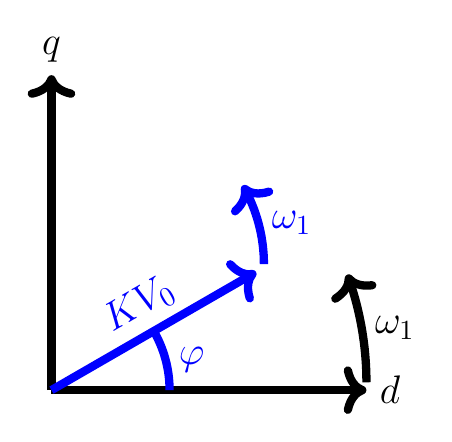
\begin{tikzpicture}[line width=3pt, font = \Large]
	\draw[->] (0,0) -- (4,0)  node[right] {$d$};
   	\draw[->] (0,0) -- (0,4)  node[above] {$q$};
   	\draw[->,blue] (0,0) -- ({3*cos(30)},{3*sin(30)})  node[midway,above,rotate=30] {$K V_0$};
   	\draw[-,blue] (1.5,0) arc (0:30:1.5) node[midway,right] {$\varphi$};
   	\draw[->,black] (4,0.1) arc (0:20:4) node[midway,right] {$\omega_1$};
   	\draw[->,blue] ({3*cos(30)+0.1},{3*sin(30)+0.1}) arc (0:30:2) node[midway,right] {$\omega_1$};
\end{tikzpicture}


\end{document}